\specialsection{Community}{}{white}{black}

\begin{figure}
	\centering
	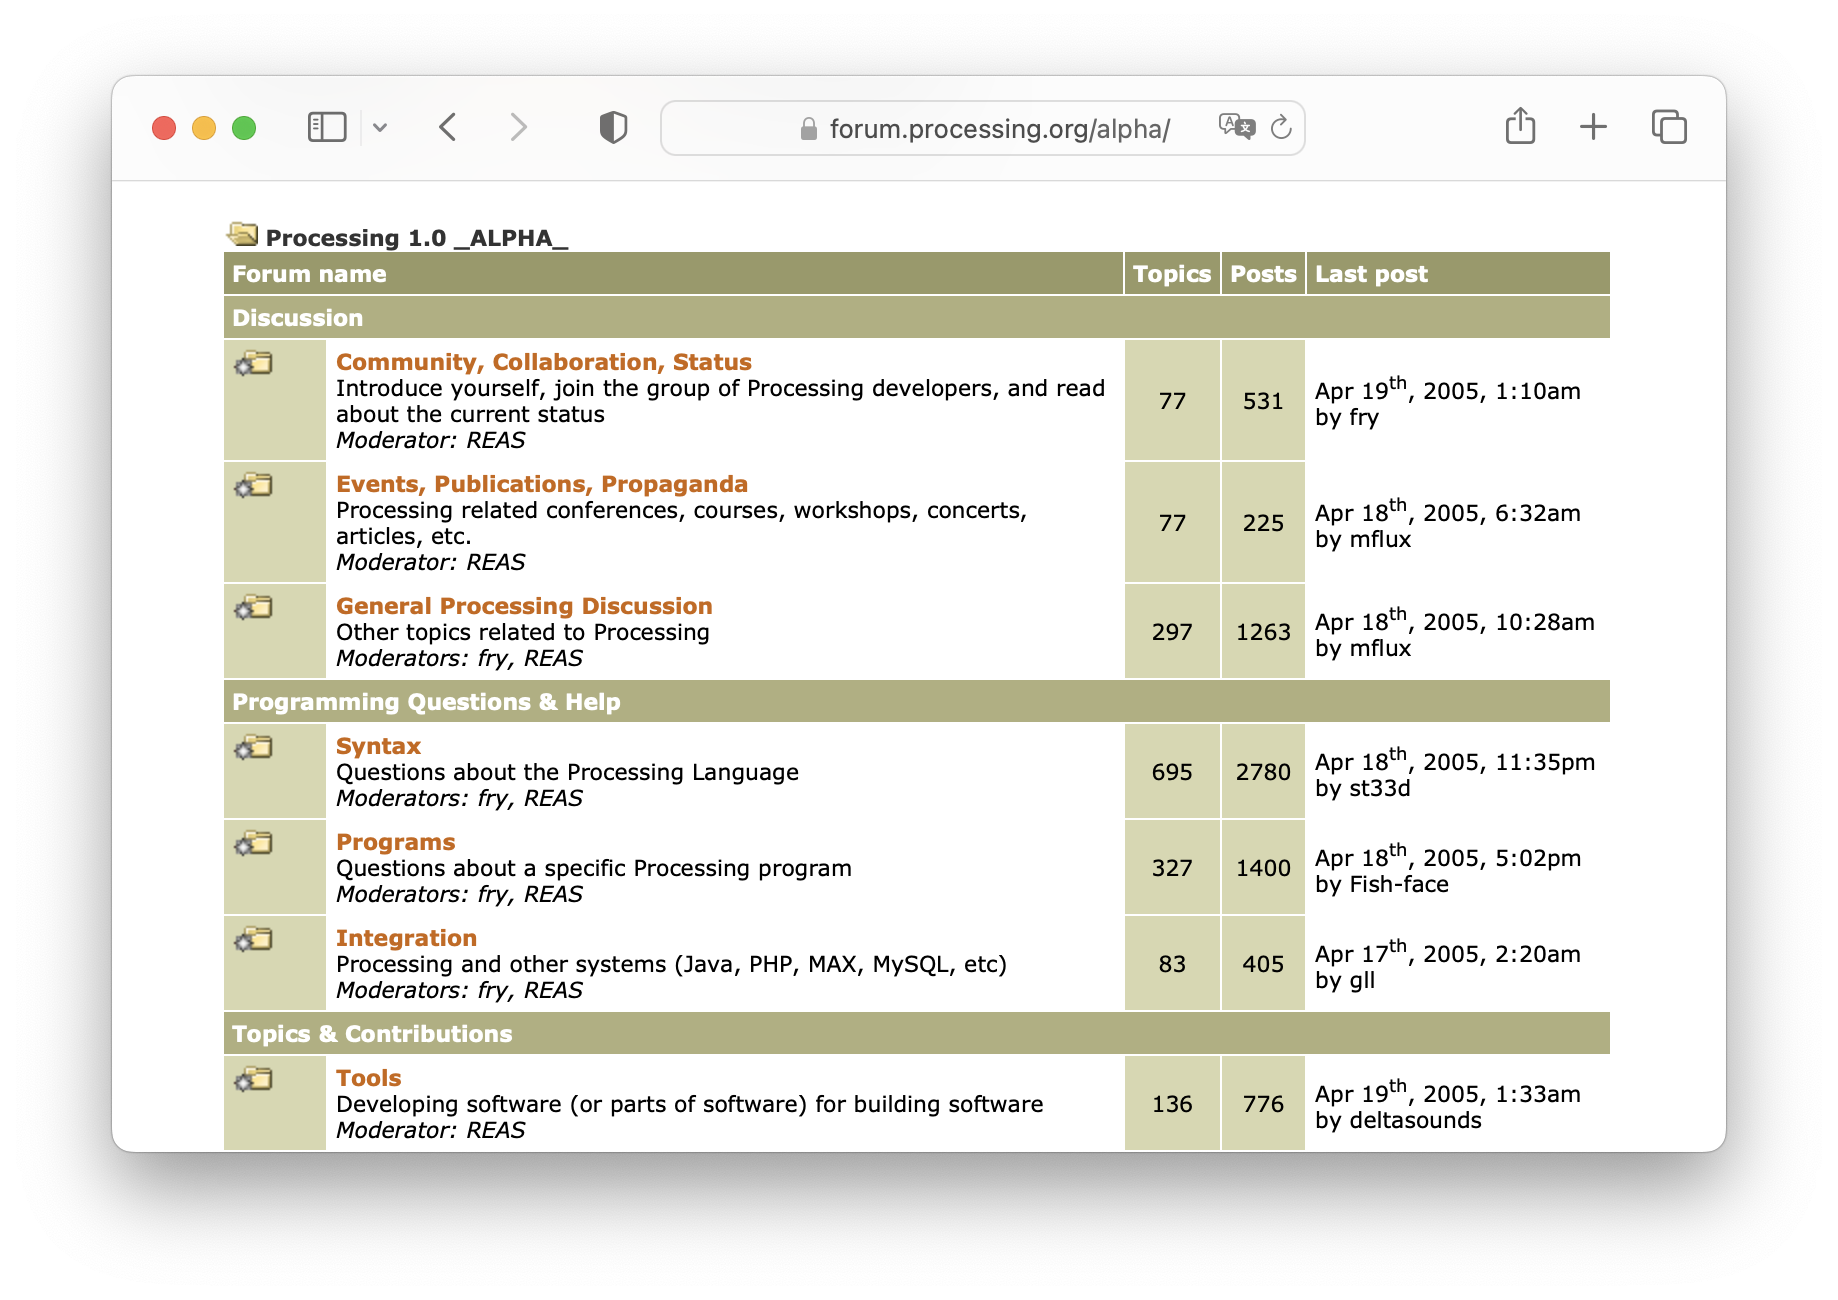
\includegraphics[width=1.0\textwidth]{images/alpha-browser.png}
	\caption{Screenshot of the Processing Alpha Forum}
	\label{fig:processing-alpha}
\end{figure}

\subsection{A community of practice}
Going beyond the technical aspects of software creation, we would like to delving into the social dynamics and learning processes that underpin the community's success.
Indeed, members of the community recognize that not only software is important as a contribution to the community “Contributors recognize that writing code is not the only way to become a contributor; they think teaching, organizing community events, and creating tutorials and documentation are valuable ways of contributing and building community. One contributor that I talked to even suggested that perhaps final users should also be considered contributors because without them there would be no reason for developing or teaching p5.js.” ([Processing Foundation, 2022, p. 41]
I believe in understaning these relathionships it is more appropriate to analyse it through a different model than that of software contributions, that is why I chose to employ the Wegner's Communities of Practice model in our analysis stems from its emphasis on learning as a communal process, a concept deeply resonant with the ethos of the Processing community, given it's focus on education. The early community, thrives on peer-to-peer interaction, collaborative discussions, and shared creative exploration. These characteristics align closely with the three fundamental elements of Wegner's model: mutual engagement, joint enterprise, and shared repertoire, but also concepts like Legitimate Periphial Participation. By applying this framework, we seek to understand how members of the Processing community engage with one another, contribute to shared goals, and develop a collective body of knowledge and practices. Albeit 

Moreover, analyzing the Processing community through the lens of the CoP model offers insights into the broader implications of community-led software development and learning. 

% Data analysis - complement other interviews
The Alpha forum was subjected to data scraping and a preliminary analysis. This process was used to identify active members for potential interviews. The forum’s significance, as underscored by Reas, was a key consideration in this analysis. Reas asserted that the forum cultivated a ‘unified international community’ from 2002 to 2006 \parencite[331]{conradGraphicDesignPostdigital2021}, further highlighting its importance. This exploration provides valuable insights into the early stages of the Processing project and its community dynamics.

% Methodology - selecting the most active forum participants
Following an analysis of the data, the most active members by the number of posts were selected for interview, namely Ariel Malka (arielm), Martin Gomez (Martin), and Jacob Schwartz (benelek). These individuals were selected for their active participation in the forum, without being a library contributor or a core developer. 

\subsection{Forum Contributors}

In exploring the dynamics of community engagement within the Processing forums, the experiences of its most active participants reveal a compelling embodiment of Wenger's concept of legitimate peripheral participation. Wenger (1998, p. 117) describes this as a journey that begins “on the periphery – a region that is neither fully inside nor fully outside” of a Community of Practice (CoP), leading progressively towards more central involvement through growing participation. This path, from initial periphery to central engagement, is vividly illustrated in the trajectories of individuals like Ariel Malka, Martin Gomez, and Jacob Schwartz, who, despite lacking local communities in their respective fields, found a sense of belonging and professional identity within the Processing community.

Jacob Schwartz’s experience within this digital CoP is particularly illustrative of this journey. Initially, Schwartz engaged with the forums as a peripheral participant, primarily observing and learning from the exchanges and projects of others. This phase of lurking and learning is crucial in the process of legitimate peripheral participation, allowing individuals to acclimatize to the community's norms, language, and practices.

Schwartz’s own words capture the essence of his evolving involvement: "I got a lot out of posting what I was working on and then getting feedback from that and also looking at what other people were working on and seeing how they did those things." This reflection not only highlights his transition from passive observation to active contribution but also underscores the reciprocal nature of learning within the community. By sharing his work, receiving feedback, and drawing inspiration from others, Schwartz moved from the periphery of the community towards a more central, contributory role.

Similarly, Ariel Malka and Martin Gomez’s narratives reflect this transformative community engagement. Malka’s deepening involvement transitioned from basic forum participation to significant contributions, such as participating in community exhibitions and testing software. Gomez, who felt isolated in his home country, found in the Processing forum a vital platform for development and collaboration, moving from a solitary enthusiast to an active community contributor.

These narratives collectively illustrate how online platforms, like the Processing forums, serve as critical enablers for legitimate peripheral participation. They provide a conduit for individuals without local communities to engage, learn, and eventually contribute meaningfully. The experiences of Malka, Gomez, and Schwartz not only shed light on the practical application of this concept but also underscore the importance of digital communities in nurturing individual growth, fostering skill development, and establishing a sense of belonging within specialized fields.

\subsection{Community Discussion Platforms}
\cleardoublepage
\changepapersize{305.3mm:210mm}
\customtag{largepage}
% \fancyhf{} % Clear all header and footer fields


% \setlength{\spiralWidth}{10.7mm}
% 147.3
\begin{minipage}{147.3mm}
{
	\LARGE
	\noindent Community Connectedness \par
}
\begin{figure}[H]
	\centering
	\includesvg[pretex=\sffamily\fontsize{5.58pt}{8pt}\selectfont, width=0.95\textwidth, keepaspectratio]{images/year.svg}
	\caption{Connectedness through forum threads of top 100 alpha forum contributos}
	\label{figure:year}
\end{figure}

\end{minipage}

\newpage
% \pagestyle{fancy}

\customtag{largepage}
\begin{minipage}[t]{0.7\textwidth}
\begin{figure}[H]
  \begin{adjustbox}{width=\textwidth, keepaspectratio}
      \begin{tabular}{cccc}
          % Row 1
          \begin{subfigure}[b]{0.24\textwidth}
              \centering
              \includesvg[width=\linewidth, keepaspectratio]{images/month1.svg}
              \caption{Month 1}
              \label{fig:month1}
          \end{subfigure} &
          \begin{subfigure}[b]{0.24\textwidth}
              \centering
              \includesvg[width=\linewidth, keepaspectratio]{images/month2.svg}
              \caption{Month 2}
              \label{fig:month2}
          \end{subfigure} &
          \begin{subfigure}[b]{0.24\textwidth}
              \centering
              \includesvg[width=\linewidth, keepaspectratio]{images/month3.svg}
              \caption{Month 3}
              \label{fig:month3}
          \end{subfigure} &
          \begin{subfigure}[b]{0.24\textwidth}
              \centering
              \includesvg[width=\linewidth, keepaspectratio]{images/month4.svg}
              \caption{Month 4}
              \label{fig:month4}
          \end{subfigure} \\
          % Row 2
          \begin{subfigure}[b]{0.24\textwidth}
              \centering
              \includesvg[width=\linewidth, keepaspectratio]{images/month5.svg}
              \caption{Month 5}
              \label{fig:month5}
          \end{subfigure} &
          \begin{subfigure}[b]{0.24\textwidth}
              \centering
              \includesvg[width=\linewidth, keepaspectratio]{images/month6.svg}
              \caption{Month 6}
              \label{fig:month6}
          \end{subfigure} &
          \begin{subfigure}[b]{0.24\textwidth}
              \centering
              \includesvg[width=\linewidth, keepaspectratio]{images/month7.svg}
              \caption{Month 7}
              \label{fig:month7}
          \end{subfigure} &
          \begin{subfigure}[b]{0.24\textwidth}
              \centering
              \includesvg[width=\linewidth, keepaspectratio]{images/month8.svg}
              \caption{Month 8}
              \label{fig:month8}
          \end{subfigure} \\
          % Row 3
          \begin{subfigure}[b]{0.24\textwidth}
              \centering
              \includesvg[width=\linewidth, keepaspectratio]{images/month9.svg}
              \caption{Month 9}
              \label{fig:month9}
          \end{subfigure} &
          \begin{subfigure}[b]{0.24\textwidth}
              \centering
              \includesvg[width=\linewidth, keepaspectratio]{images/month10.svg}
              \caption{Month 10}
              \label{fig:month10}
          \end{subfigure} &
          \begin{subfigure}[b]{0.24\textwidth}
              \centering
              \includesvg[width=\linewidth, keepaspectratio]{images/month11.svg}
              \caption{Month 11}
              \label{fig:month11}
          \end{subfigure} &
          \begin{subfigure}[b]{0.24\textwidth}
              \centering
              \includesvg[width=\linewidth, keepaspectratio]{images/month12.svg}
              \caption{Month 12}
              \label{fig:month12}
          \end{subfigure}
      \end{tabular}
  \end{adjustbox}
  \caption{First year of the Alpha forum}
  \label{fig:monthlyGraphs}
\end{figure}
\end{minipage}
\hfill
\begin{minipage}[t]{0.25\textwidth}
  \vspace{8mm}
  \small
  The Alpha forum's developmental trajectory over its first year, as visualized through network graphs, reveals a dynamic growth narrative. Initially, a compact hub of activity signals robust engagement from a committed group of participants, laying the groundwork for the community's expansion. This is evidenced by an increase in the density and reach of interactions, suggesting a broadening in the diversity of contributors and a rise in active membership. The persistent complexity of the network and uniform distribution of connections throughout the year highlight an environment where individuals are actively integrated, promoting a collective and inclusive exchange of knowledge.

  \medskip
  The absence of isolated clusters within these visualizations speaks to a forum culture that successfully assimilates newcomers into the ongoing dialogue, maintaining an equitable and collaborative discourse. This enduring interactivity, underscores the forum's efficacy as a thriving digital ecosystem conducive to sustained collaboration and exchange.

\end{minipage}

\defaultareasettings

%\begin{figure}[h!] 
    \centering 
    \includesvg[pretex=\sffamily\fontsize{5.58pt}{8pt}\selectfont, width=1\textwidth, keepaspectratio]{images/figure-forum-posts.svg}
    \caption{Top 12 authors by number of posts (Aggregated alpha and beta forum)}
    \label{fig:forum-posts}  
  \end{figure}
%\begin{figure}[htbp] 
    \centering
    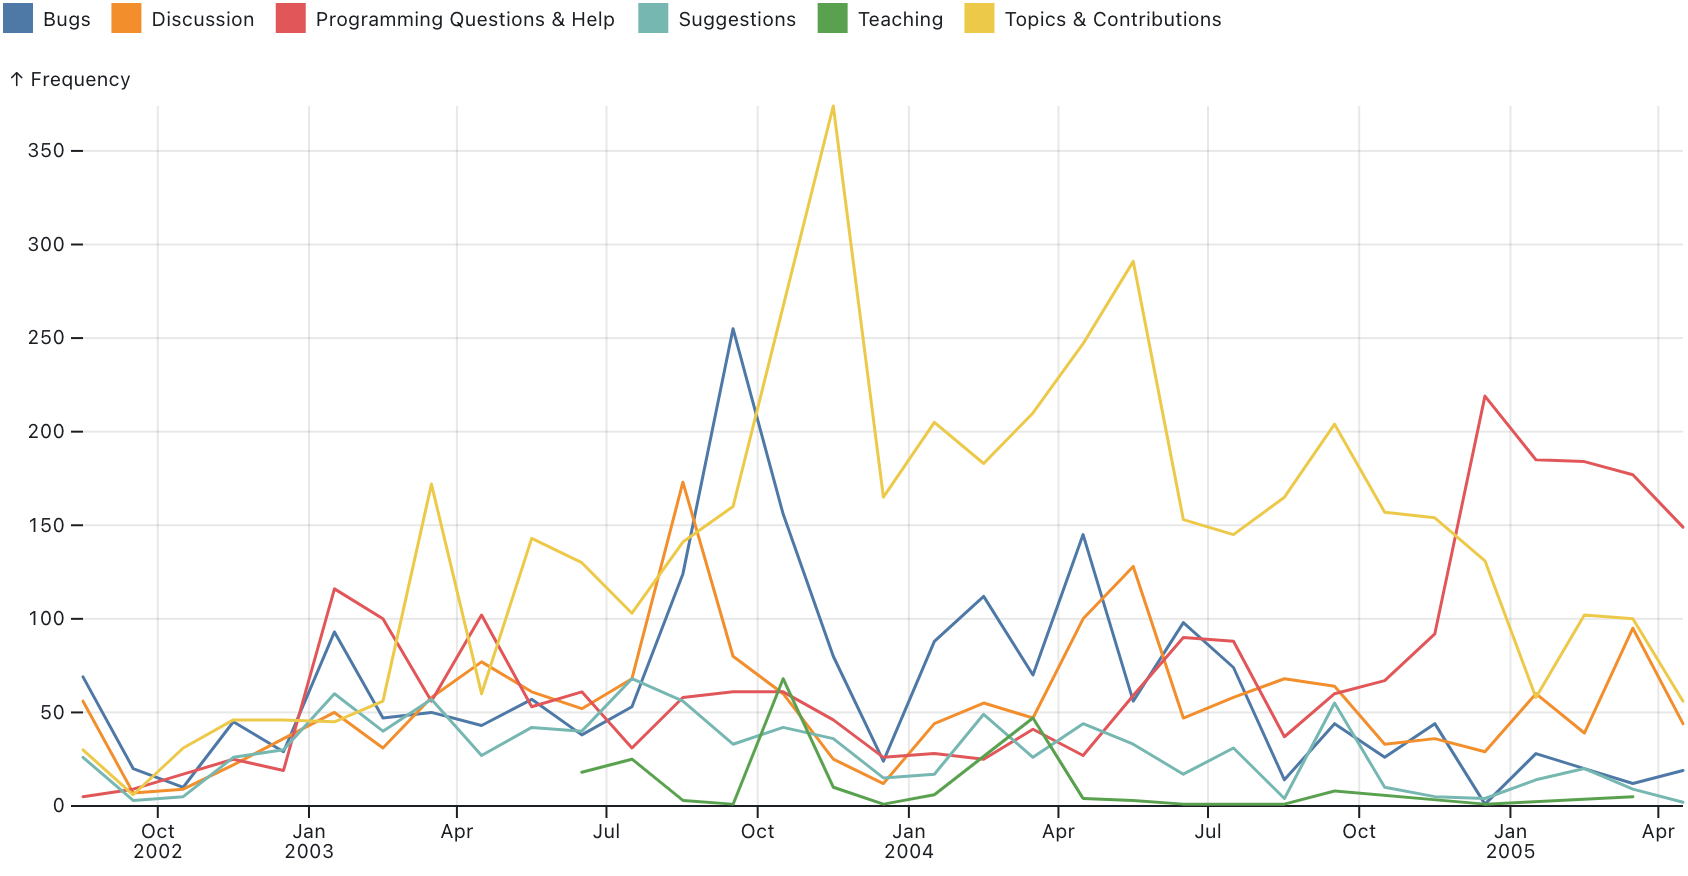
\includegraphics[width=1\textwidth]{alpha-forums-activity.png} 
    % \includesvg[pretex=\sffamily\fontsize{5.58pt}{8pt}\selectfont, width=0.6\textwidth]{images/alpha-forums-activity.svg}
    \caption{Forums activity}
    \label{fig:forum-activity}  
  \end{figure}
%\begin{figure}[h!] 
    \centering 
    \includesvg[pretex=\sffamily\fontsize{5.58pt}{8pt}\selectfont, width=1\textwidth, keepaspectratio]{images/figure-alltime-sourcecode-commits.svg}
    \caption{Top 25 source code contributors by number of commits}
    \label{fig:alltime-sourcecode-commits}  
  \end{figure}
%\begin{figure}[htbp] 
    \centering
    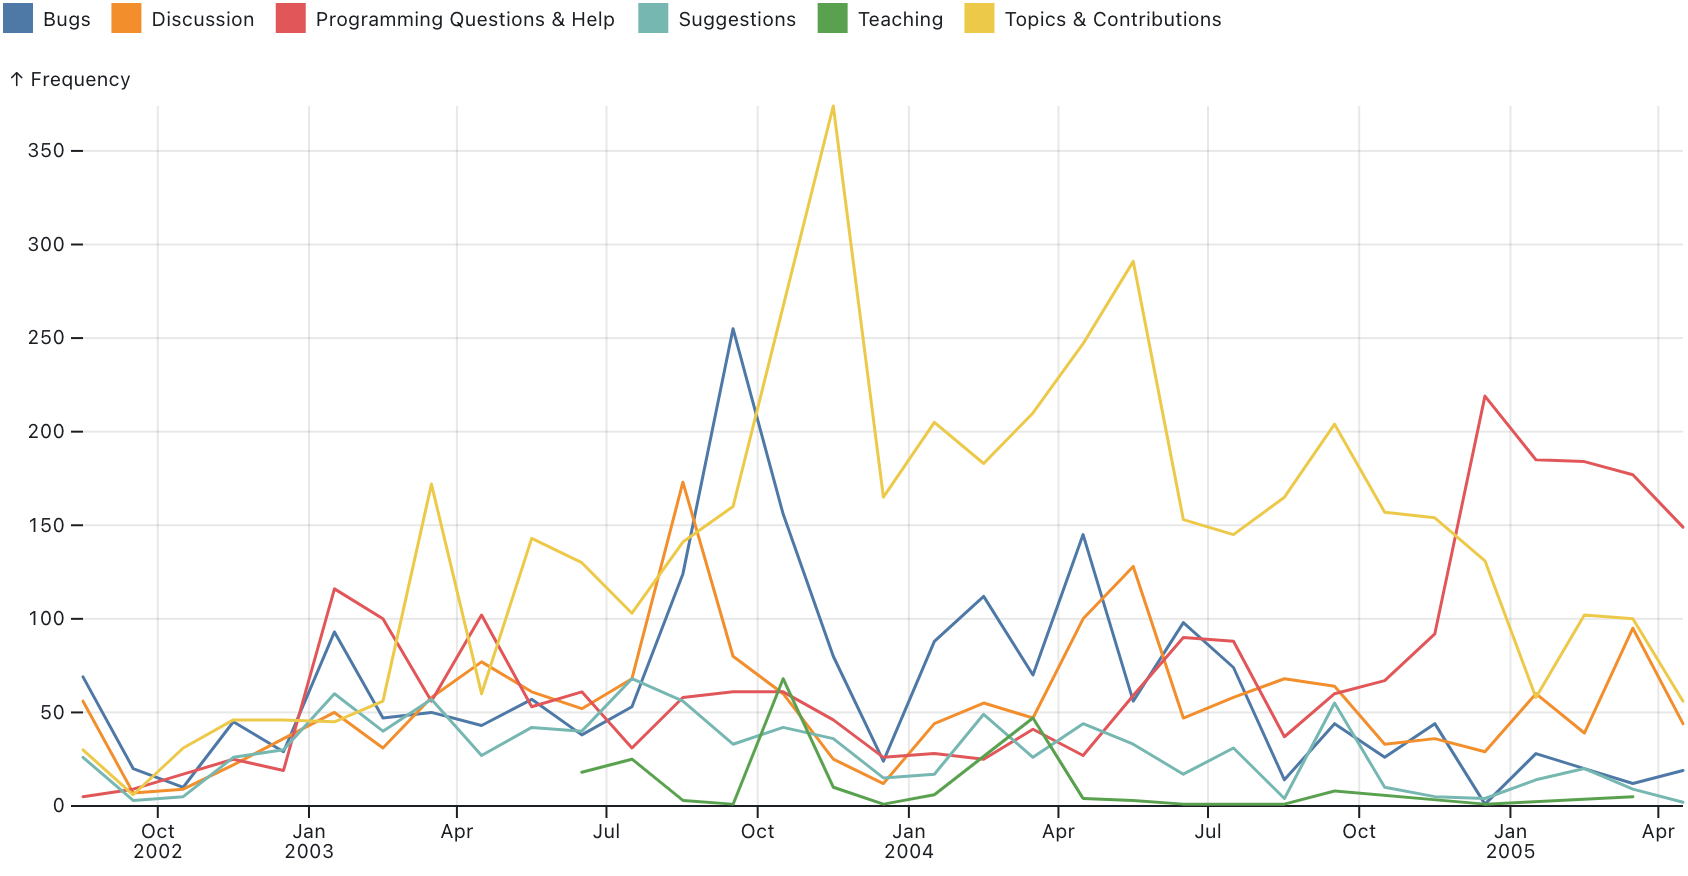
\includegraphics[width=1\textwidth]{alpha-forums-activity.png} 
    % \includesvg[pretex=\sffamily\fontsize{5.58pt}{8pt}\selectfont, width=0.6\textwidth]{images/alpha-forums-activity.svg}
    \caption{Forums activity}
    \label{fig:forum-activity}  
  \end{figure}

\begin{figure}
    \centering 
    \includesvg[pretex=\sffamily\fontsize{5.58pt}{8pt}\selectfont, width=1\textwidth, keepaspectratio]{images/alpha-forums-by-posts.svg}
    \caption{Topics by post number}
    \label{fig:forums}  
  \end{figure}
\begin{table}[h]
	\raggedright
	\begin{adjustbox}{center}
		\begin{tabular}{l l l c}
			\toprule
			Forum name                   & Years      & URL                                                                    \\
			\midrule
			Processing alpha forum       & 2002-2005  & \href{https://forum.processing.org/alpha/}{forum.processing.org/alpha} \\
			Processing beta forum        & 2005-2010  & \href{https://forum.processing.org/beta/}{forum.processing.org/beta}   \\
			Processing 1.0 forum         & 2010-2013  & \href{https://forum.processing.org/one/}{forum.processing.org/one}     \\
			Processing 2.0 and 3.0 forum & 2013-2018  & \href{https://forum.processing.org/two/}{forum.processing.org/two}     \\
			Current processing forum     & 2018 - now & \href{https://discourse.processing.org/}{discourse.processing.org}     \\
			\bottomrule
		\end{tabular}
	\end{adjustbox}
	\caption{Archival forums composition}
	\label{table:forums}
\end{table}
% Interviews
% Library and code contributors
% graph of the alpha forum contributors

\newpage
\begin{figure}
	\centering
	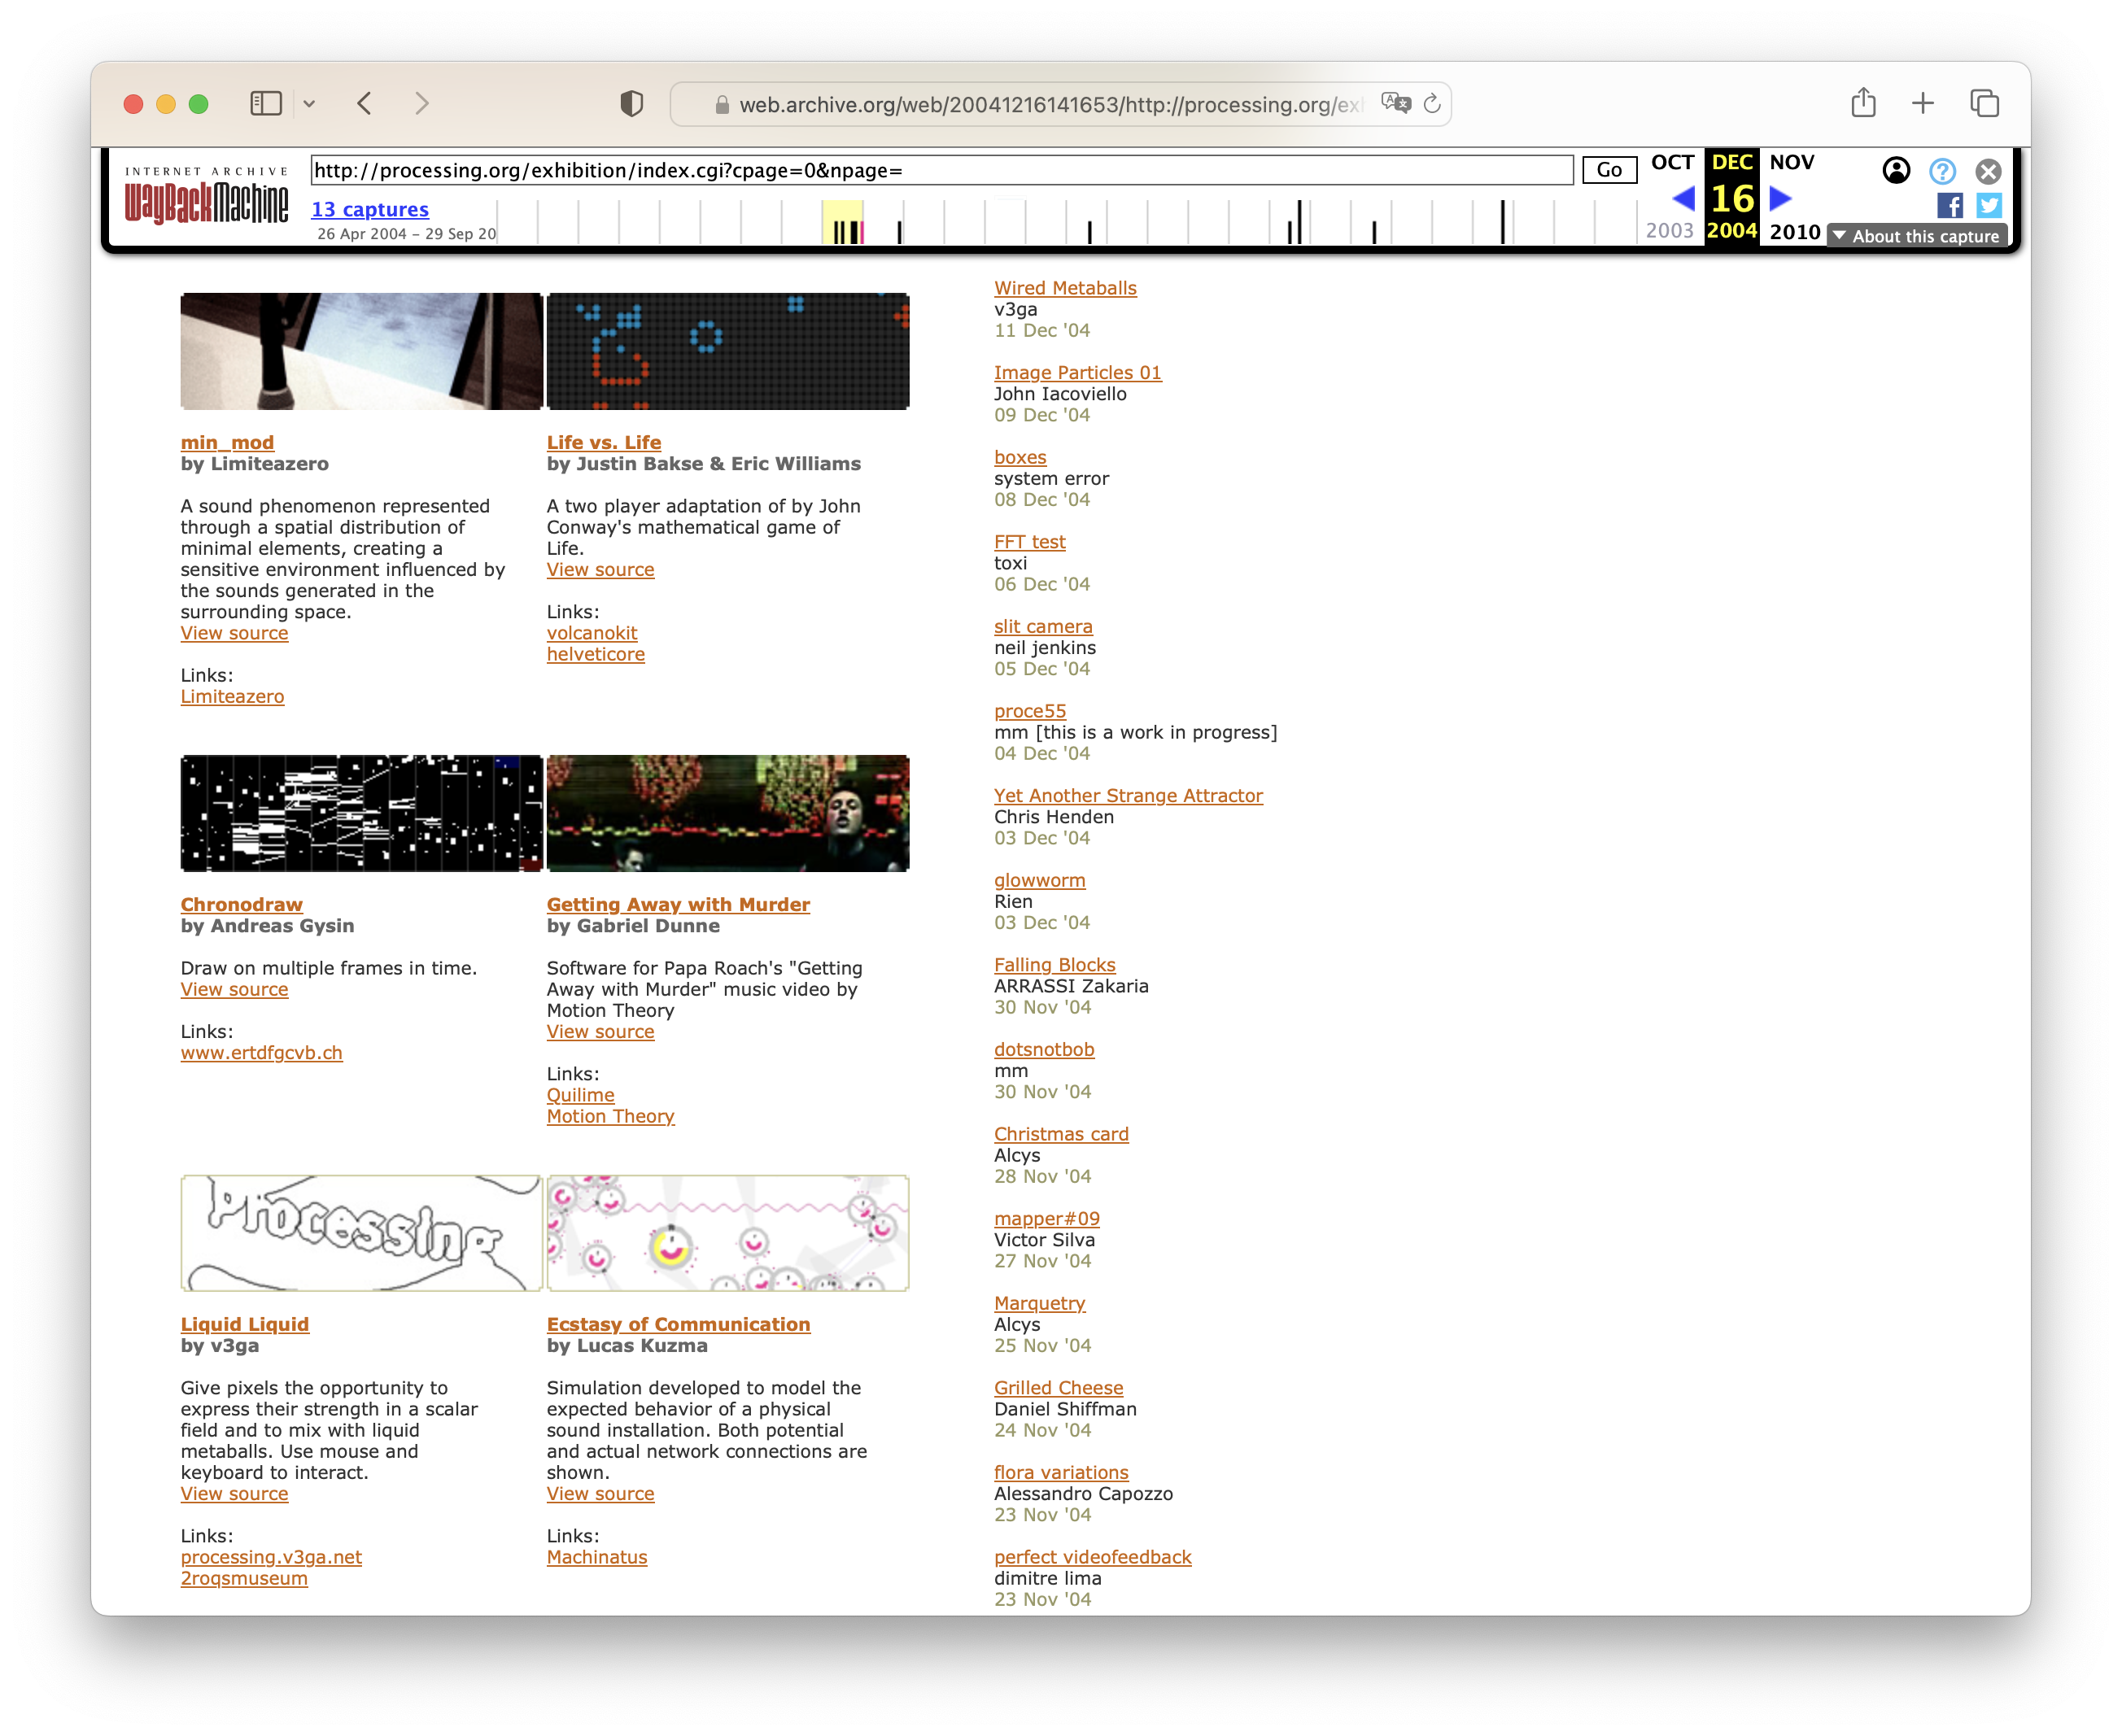
\includegraphics[width=1.0\textwidth]{images/exhibitions.png}
	\caption{Screenshot of community exhibition}
	\label{fig:website-exhibition}
\end{figure}

\subsection{Elements of Community Engagement}

The Processing community, characterized by its shared repertoire, demonstrates a unique cohesion through communal resources, encompassing tools, concepts, methods, and standards. Central to this repertoire is the Processing environment itself, a common tool and language that has been instrumental in cultivating a keen interest in Computational Design. This shared platform has enabled members to effectively communicate and exchange code, fostering a collaborative spirit.

One notable aspect of this shared repertoire is the emphasis on providing minimal working examples or prototypical programs, complete with demonstrations of project capabilities. This culture of crafting and sharing concise yet illustrative examples was a distinctive trait of the Processing community, highlighting their focus on practical, user-friendly, and educational resources.

The Processing community gained recognition for its practice of showcasing member works on the exhibition page of its website. This approach encouraged not only code sharing but also a sense of inspiration within the community. The initial projects published by founders Fry and Reas played a crucial role, sparking discussions in forums and intensifying interest in Processing. The community's culture of sharing and inspiration, illustrated by examples like Ariel Malka's chronotext project and Glen Murphy's influence on Ricard Marxer, will be further explored, along with Ben Fry's commentary on how these dynamics contributed to community growth.

Forum interactions in the Processing community also mirrored this ethos of shared learning and collaboration. Members frequently posted codes and detailed explanations on websites, facilitating knowledge exchange. The following is an exemplar forum post by Glen Murphy, illustrating this culture of sharing and constructive feedback:

-----
Glen Murphy

WWW Email
Fluid Dynamics
« on: Nov 5th, 2002, 12:49pm »	
Fluid 3: http://bodytag.org/nav.php?u=fluid3/
 
Fluid 3 Source: http://bodytag.org/fluid3/fluid3.pde
 
+
 
Smoke 2: http://bodytag.org/nav.php?u=smoke2/
 
Smoke 2 Source: http://bodytag.org/smoke2/smoke2.pde
 
--
Neither of these are 'full' fluid simulations. For example, Navier-Stokes is nowhere to be seen, and the pressure calculations are pretty raw.
 
May be useful as a base for something.
---------------


The encouragement to share and create for the community exhibition page fostered a transparent environment where members were aware of others' expertise and could readily seek assistance. Ariel Malka specifically mentioned the motivational aspect of this platform for his engagement.

In addition to technical discussions, philosophical debates also found a place within the community. An example is a forum topic discussing the relationship between code and art, showcasing the intellectual depth of the community members:

% -------
% Author	 Topic: code != art  (Read 3018 times)
% Martin

% 122417302122417302martingomez_listsmg1ph WWW Email
% code != art
% « on: Apr 19th, 2003, 7:05pm »	
% there exists some written work and live people who preach that code is not art, nor should code be considered to realize the soul of digital art. what's your take on this?
% --------

In conclusion, the shared repertoire of the Processing community, manifested through its common language, culture of example crafting, exhibition page, forum interactions, and intellectual debates, significantly contributed to its development and identity. This collaborative and open environment not only facilitated technical skill development but also fostered a rich, philosophical dialogue among its members.

Joint Enterprise
Collective Goals and Objectives: Centers on the shared goals and visions that drive the community's collective efforts.

Karsten Schmidt emphasized the communal aspect of open-source projects and the expectation of contribution as part of being in such communities: "I think when you sign up to use open source tooling, you make a kind of social agreement to be part of that culture as well, which gives you so much that there should be a kind of social expectation to also want to give something back."

Ricard Marxer reflected on the open-source community's dynamics, indicating a shared responsibility: "Every time that somebody would use it or would point out maybe some mistake, you said, Oh, then people are really relying on this. So you try to fix the mistake and put it into the next version."



Similarly joint enterprise was 

Impact and Influence on Broader Fields: Looks at how the community's joint efforts extend their influence beyond their immediate domain.
- Martin Gomez story of making exhibitions in the Phillipines, where computational desgin was not really known

% ##### 

In exploring the mutual engagement within the early Processing community, a concept central to Wenger's theory, we observe a dynamic interplay of collaboration, individual contributions, and supportive feedback mechanisms. This community, as it evolved, displayed a rich tapestry of interactions and personal involvements that underpin the essence of a thriving community of practice.

The collaboration and interaction within the Processing community were not merely incidental but formed the bedrock of its growth and development. Jacob Schwartz's reflection on his engagement with the community captures this essence: "I would say that the tool itself was very interesting to me, but the community was a huge part of it for me as well." This perspective highlights the symbiotic relationship between individual and collective pursuits, where personal interests are entwined with communal activities. This environment of shared learning and collaboration is further illuminated by Karsten Schmidt's recollections, depicting a collective journey of discovery and understanding within the community, a hallmark of mutual engagement.

Intertwined with this collaborative spirit were the individual contributions and roles that each member brought to the community. The diversity of these contributions, ranging from code development to knowledge sharing, as exemplified by Martin Gomez's involvement, enriched the community's collective expertise. Ariel Malka's experience adds another layer to this narrative, showcasing a community that not only thrived on collective contributions but also recognized and celebrated the uniqueness of individual experiences and skills. Such a mosaic of roles and contributions reflects a vibrant community where mutual engagement fosters a rich, multifaceted practice.

Underpinning these aspects of collaboration and individuality was a robust support system and a culture of constructive feedback. Jacob Schwartz's experiences with posting his work and receiving feedback underline a community keen on nurturing growth and learning among its members. The Processing forums, as Martin Gomez observed, were a testament to this supportive ethos, where learning and understanding were the shared goals, resonating with the core principles of mutual engagement as defined by Wenger.

Karsten Schmidt: "I can't remember he was, there was a 13 year old dude on there, but he was super helpful. in the beginning it was a very small group, and everyone was really learning together what this thing is, or what it could do, and like someone did something interesting, then also How was it done? And, what are the learnings? How can we, maybe some of that stuff can be extracted into the actual to order? Maybe the tool can be changed in the future to make those things more possible, like those kind of conversations. And I've absolutely enjoyed them"​​.


\subsection{Processing Foundation}

The Processing Foundation was established in 2012 by Casey Reas, Ben Fry, and Daniel Shiffman with the primary objective of sustaining the software's development and broadening its reach. According to Fry and Reas, ``The vast majority of the code is written by the same small number of people volunteering their time — there are no paid full-time developers'' \parencite[p.~13]{fryModernPrometheusHistory2018}.

\begin{figure}[h]
	\centering
	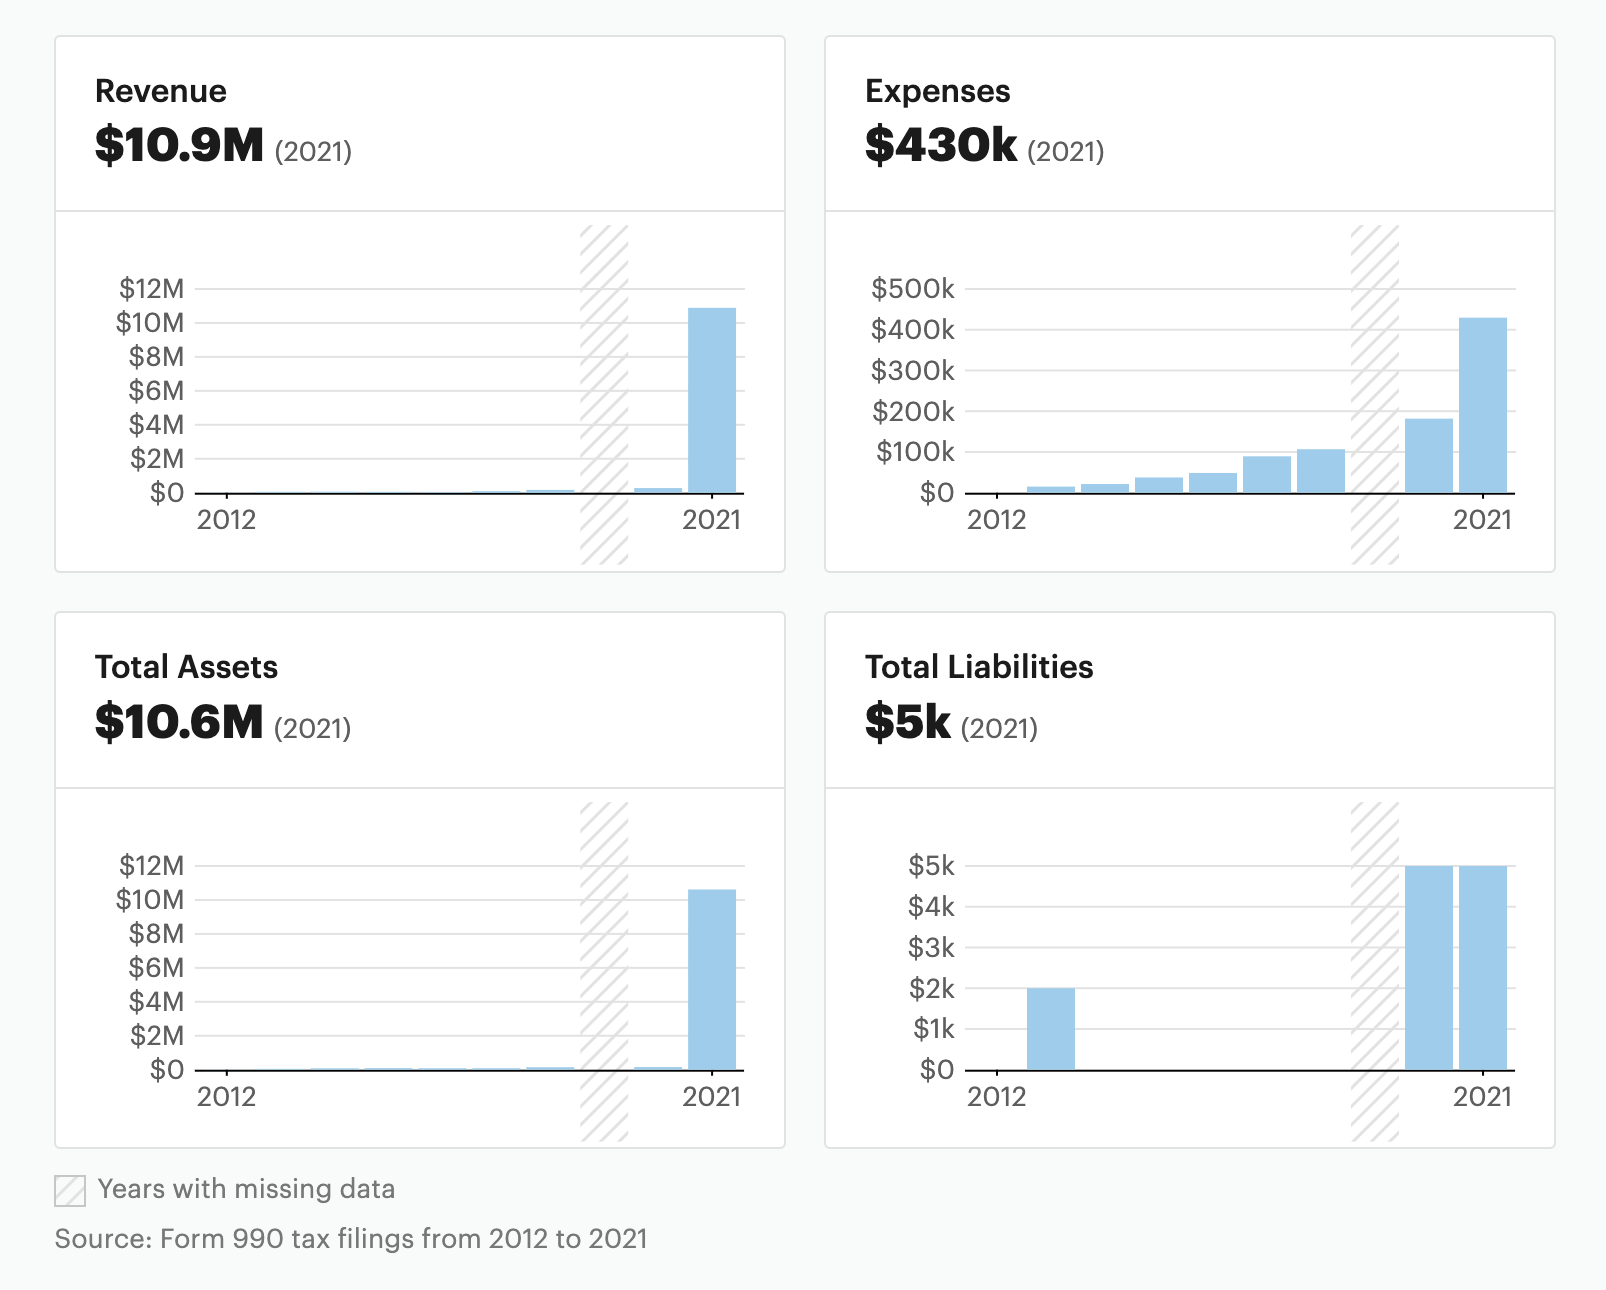
\includegraphics[width=0.9\textwidth]{images/foundation-finances.png}
	\caption{Financial growth of the Processing Foundation over the years Source: \parencite{ProcessingFoundationNonprofit2013}}
	\label{fig:foundation-finances}
\end{figure}

As shown in Figure~\ref{fig:foundation-finances}, the foundation's revenue has experienced modest growth, increasing from \$11,235 to \$273,520. Remarkably, it reached a peak revenue of \$10,889,998 in the fiscal year 2021. Throughout its history, the principal source of funding for the foundation has predominantly come from contributions.

However, the allocation of these funds has been a point of contention within the organization. Most notably, a public disagreement in 2023 led to the resignation of Ben Fry, a long-standing board member and contributor. It should be noted that Fry's perspective on the matter was not universally accepted among the foundation's other founding members. \parencite{benfry[@ben_fry]HaveMadeExtremely2023} \parencite{caseyreas[@reas]EarlierThisWeek2023} \parencite{danielshiffman[@shiffman]WouldPostNote2023}

\subsection{Community Dynamics}


